\documentclass{standalone}
\usepackage{tikz}
\usetikzlibrary{automata, positioning, arrows}

\begin{document}
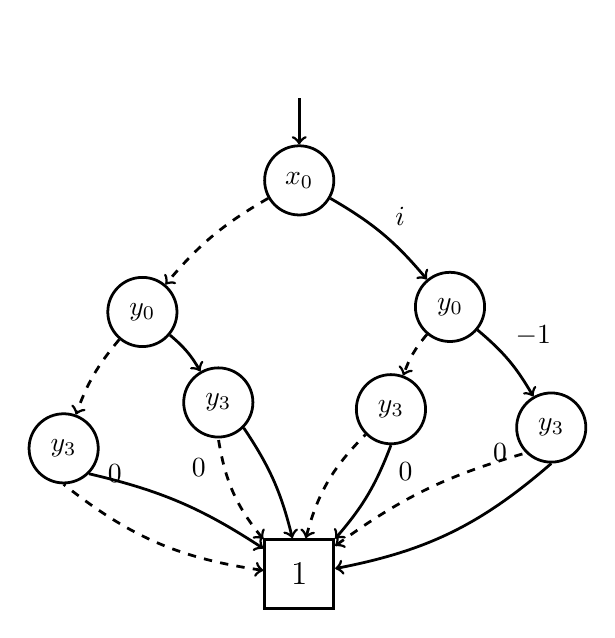
\begin{tikzpicture}[auto,node distance=1.5cm,every node/.style={shape=circle , align=center,solid,minimum size =0.01cm},line width =1pt]
  \tikzstyle{every state}=[fill=white,draw=black,text=black]

  \node[state] (A) {$x_0$};
  \node[state] (B) at ([shift = ({220:2.6cm})]A) {$y_0$};
  \node[state] (C) at ([shift = ({-40:2.5cm})]A) {$y_0$};
  \node[state] (D) at ([shift = ({240:2cm})]B) {$y_3$};
  \node[state] (E) at ([shift = ({-50:1.5cm})]B) {$y_3$};
  \node[state] (F) at ([shift = ({240:1.5cm})]C) {$y_3$};
  \node[state] (G) at ([shift = ({-50:2cm})]C) {$y_3$};
  \node[state,shape = rectangle] (H) at ([shift = ({-90:5cm})]A) {\large$1$};
  \node[state,draw=none] (I) [above of= A]       {};

  \path[->]
  (A) edge[bend right=10,dashed]  node {} (B)
  (A) edge[bend left=10]  node {$i$} (C)
  (B) edge[bend right=10,dashed]  node {} (D)
  (B) edge[bend left=10]  node {} (E)
  (C) edge[bend right=10,dashed]  node {} (F)
  (C) edge[bend left=10]  node {$-1$} (G)
  (I) edge node{} (A);
  \path[<-]
  (H) edge[bend left=15,dashed]  node {} (D.south)
  (H) edge[bend right=10]  node [at end,right] {$0$} (D.south east)
  (H) edge[bend left=15,dashed] node [near end,left] {$0$} (E.south)
  (H) edge[bend right=10]  node {} (E.south east)
  (H) edge[bend left=15,dashed]  node {} (F.south west)
  (H) edge[bend right=10]  node [near end,right] {$0$} (F.south)
  (H) edge[bend left=10,dashed]  node [at end,left] {$0$} (G.south west)
  (H) edge[bend right=15]  node {} (G.south);
\end{tikzpicture}
\end{document}